\chapter{Folosirea modelelor antrenate}
\label{chapter5}
\section{Deplasarea cursorului}
Funcționalitatea de bază a mouse-ului constă în deplasarea cursorului pe ecran.
Am implementat, în primul rând, deplasarea acestuia pe 8 direcții: N, NE, E, SE, S, SV, V, NV.
Dacă utilizatorul vrea să mute cursorul în direcția stânga-sus, atunci acesta va trebui să se uite în acea parte a ecranului (corespunzătoare celulei cu numărul 0 pe o grilă de dimensiune 3x3).
Analog, pentru a-l deplasa în sus, va trebui să se uite pe centrul ecranului în partea de sus (celula cu numărul 1) ș.a.m.d.

\begin{figure}[H]
    \centering
    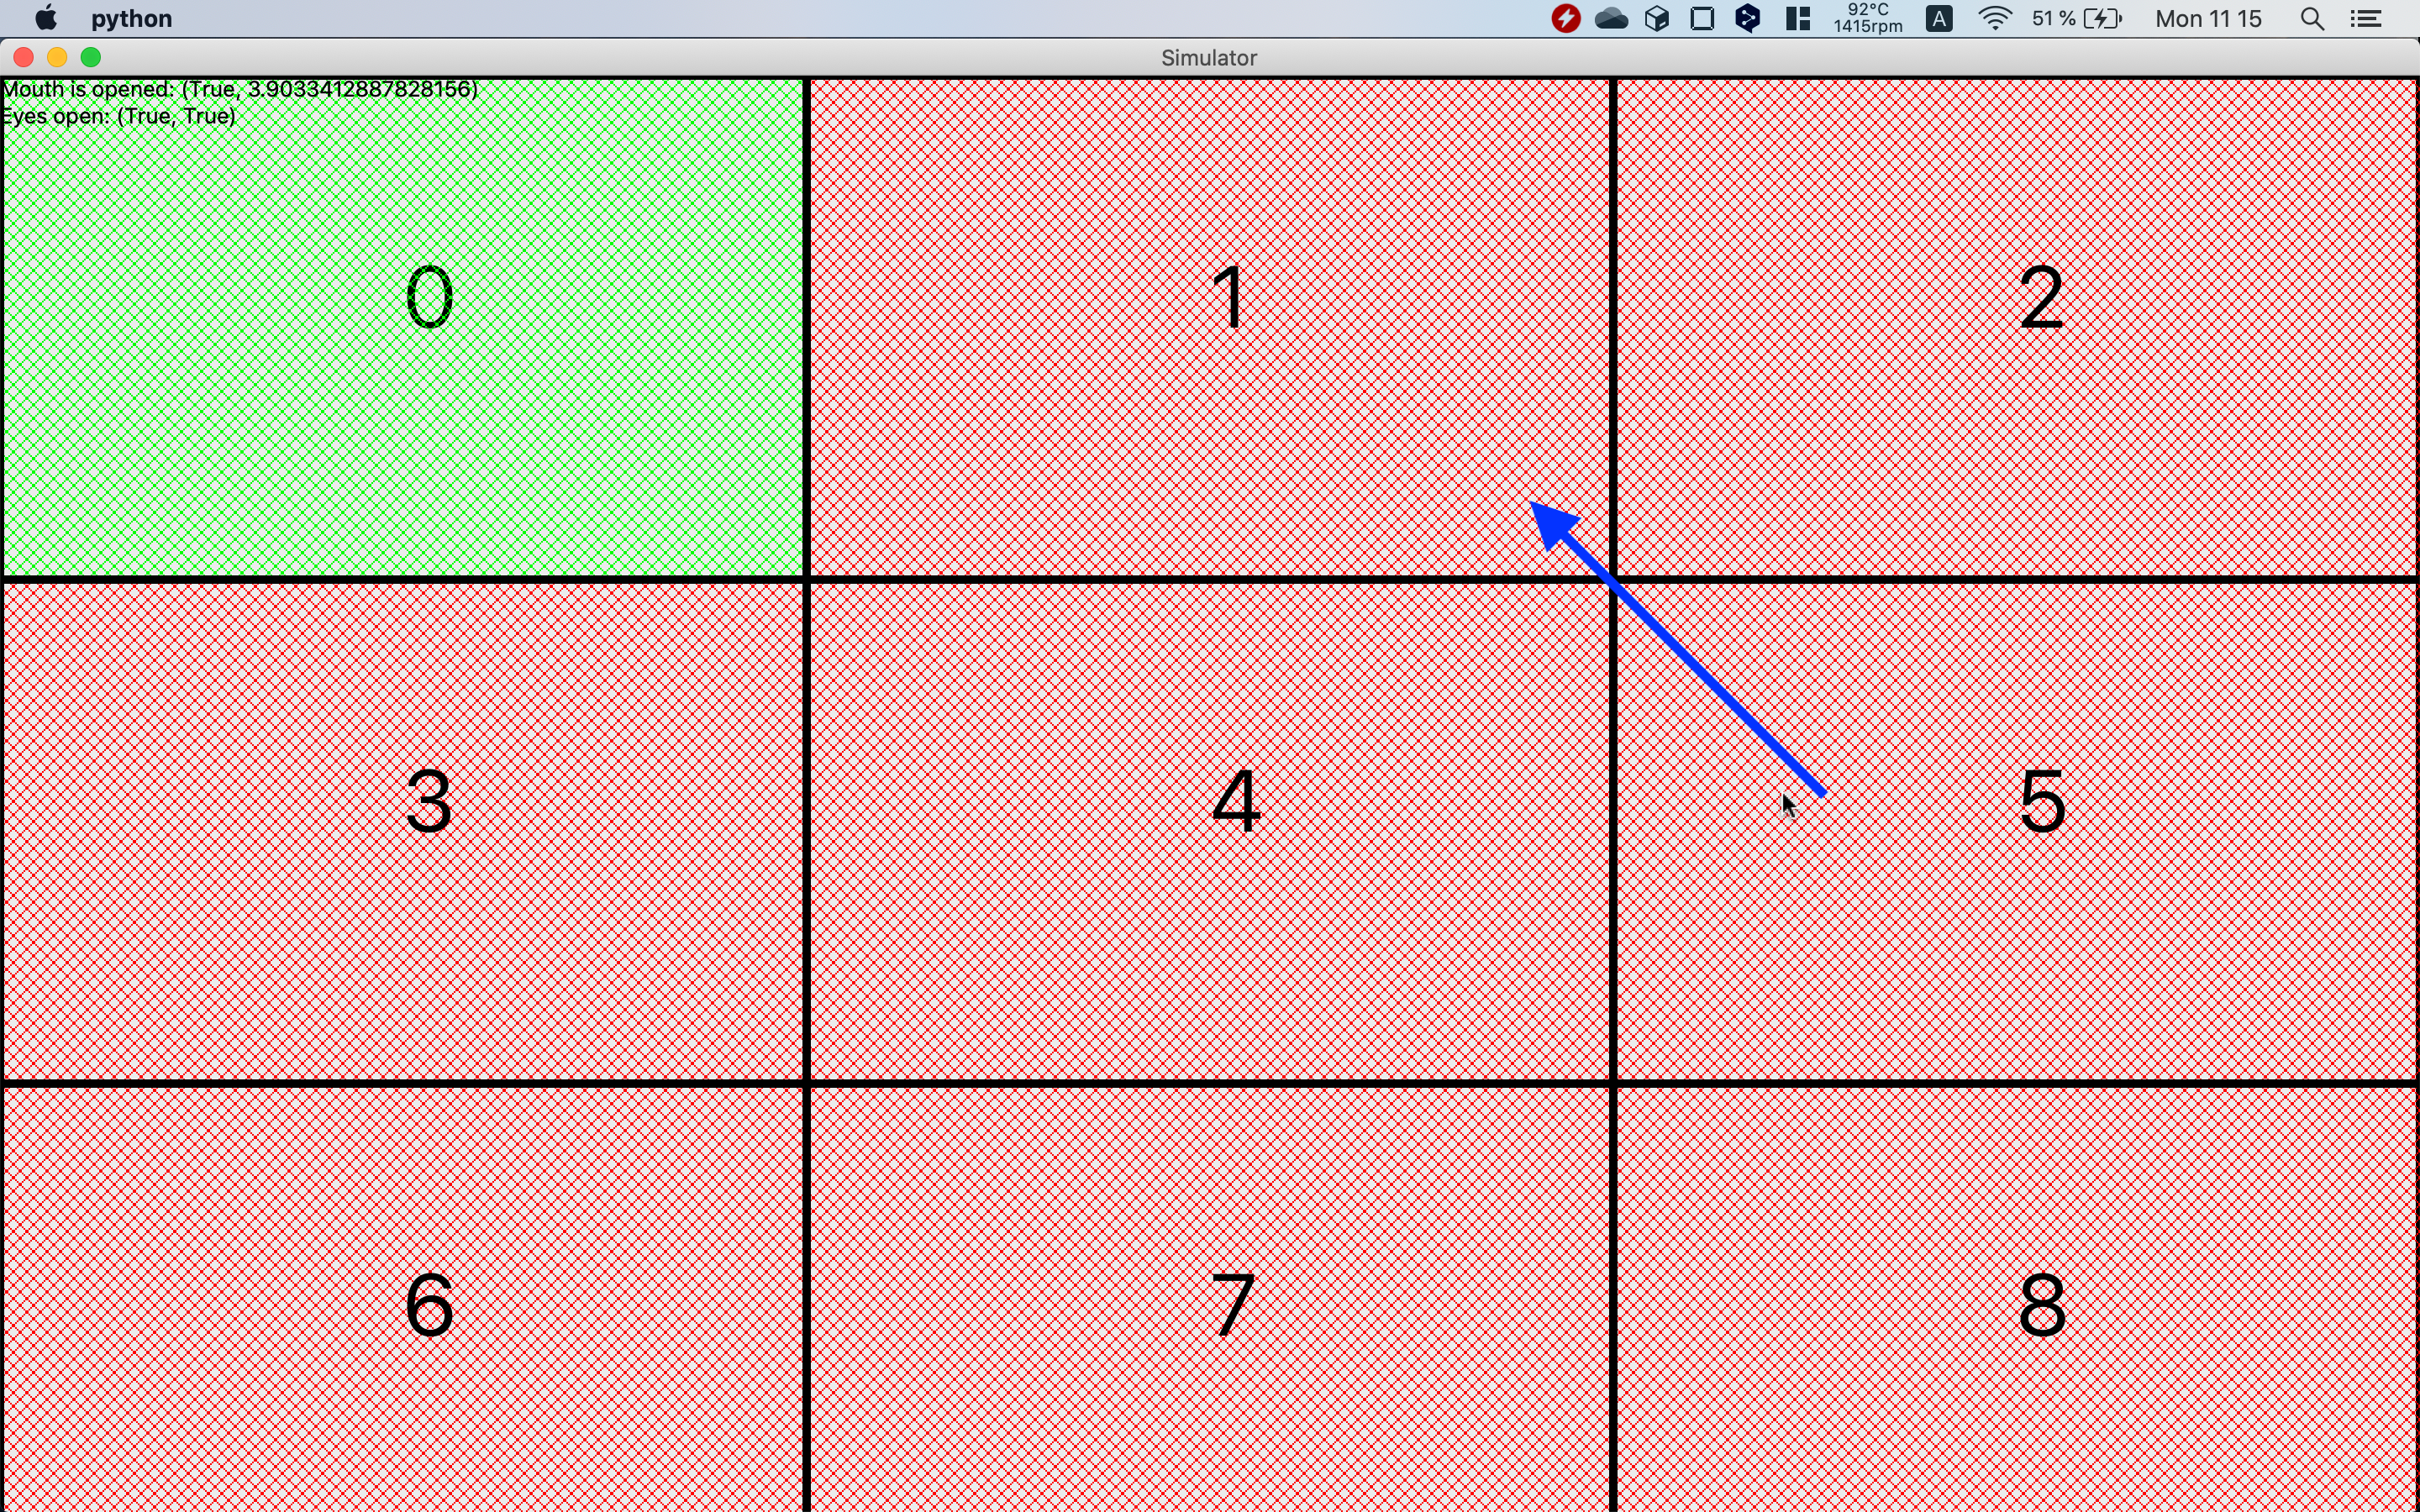
\includegraphics[width=0.7\textwidth]{cursor_movement.png}
    \caption{Deplasarea cursorului în direcția NV}
\end{figure}

Întrebarea care reiese din paragraful de mai sus este: cum poate solicita utilizatorul deplasarea cursorului?
Fiind o aplicație care se bazează doar pe gesturi ale feței, am decis ca deplasarea cursorului să se realizeze în momentul deschiderii gurii.

Un articol interesant (\cite{driver_drowsiness}) prezintă metode de identificare a oboselii unui șofer.
Un factor cheie este detectarea căscatului, care se rezumă la același gest pe care a trebuit să îl identific și eu.
Articolul propune folosirea reperelor faciale situate pe buze pentru a detecta un raportul de aspect al gurii (\emph{MAR, Mouth Aspect Ratio}).
Formula propusă este:
$$MAR = \frac{|CD| + |EF| + |GH|}{3|AB|}$$

\begin{figure}[H]
    \centering
    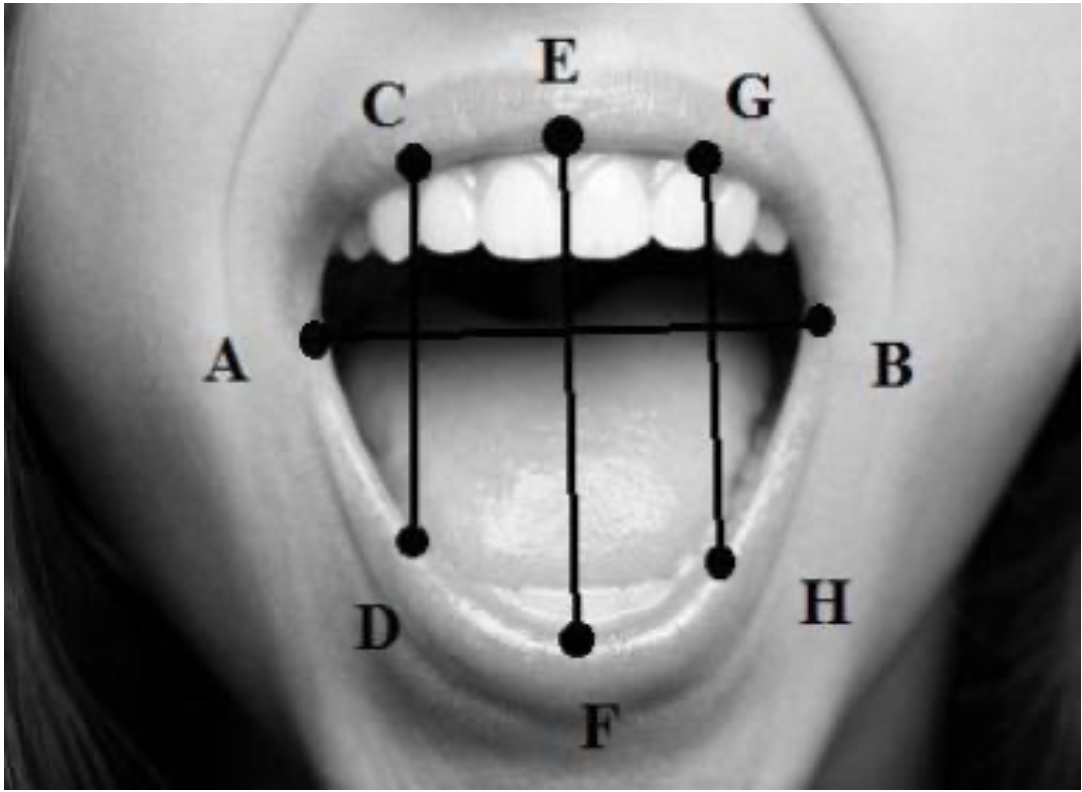
\includegraphics[width=0.3\textwidth]{mar.png}
    \caption{Repere faciale folosite pentru a calcula valoarea MAR. Imagine preluată din \cite{driver_drowsiness}}
\end{figure}

Astfel, daca valoarea \emph{MAR} depășește un anumit prag (\emph{MAR threshold}) care este configurabil, atunci aplicația consideră că acesta solicită deplasarea cursorului.
Avantajul configurării acestui prag este că poate fi setat astfel încât utilizatorul să poată și conversa în timp ce aplicația este deschisă, fără a mișca accidental mouse-ul.

\section{Apăsarea butoanelor mouse-ului}
Un gest util ce poate fi folosit în același fel ca mai sus este închiderea ochiului.
Am decis să folosesc închiderea ochiului pentru a simula funcțtiile de ``click stânga'' și ``click dreapta''.
\cite{blink_detection} propune un calcul al raportului de aspect al ochiului (\emph{EAR, Eye Aspect Ratio}) pentru a detecta când o persoană are ochiul închis sau nu.
Formula propusă este:
$$MAR = \frac{||p_2 - p_6|| + ||p_3 - p_5||}{2||p_1 - p_4||}$$

% \begin{figure}[ht]
%     \centering
%     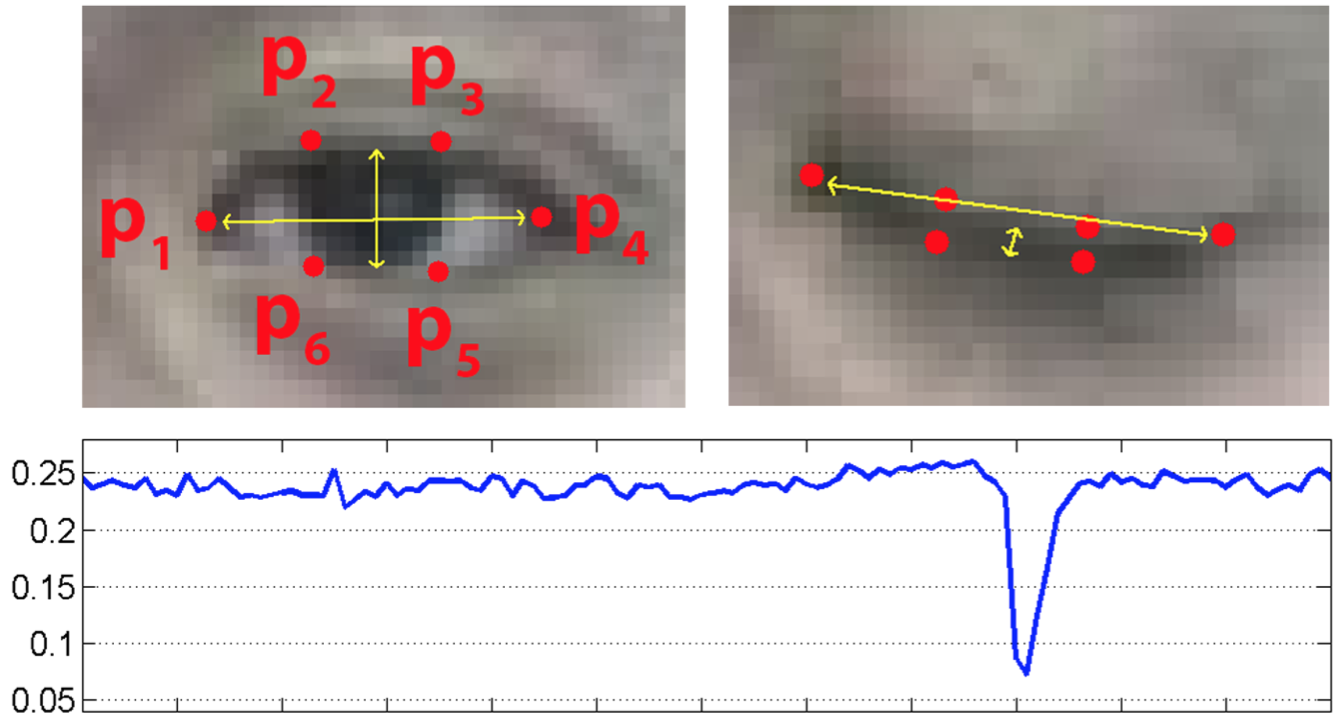
\includegraphics[width=0.5\textwidth]{ear.png}
%     \caption{Detectarea clipirii folosind valoarea EAR. Imagine preluată din \cite{blink_detection}}
% \end{figure}

Când utilizatorul menține ochiul stâng închis pentru un anumit interval de timp $\delta_t$, aplicația va efectua simularea apăsării butonului stâng.
Analog, închiderea ochiului drept va determina simularea apăsării butonului drept.
Intervalul de timp $\delta_t$ a fost folosit pentru a evita apăsarea butoanelor într-un mod inutil atunci când utilizatorul doar clipește.

\begin{figure}[H]
    \centering
    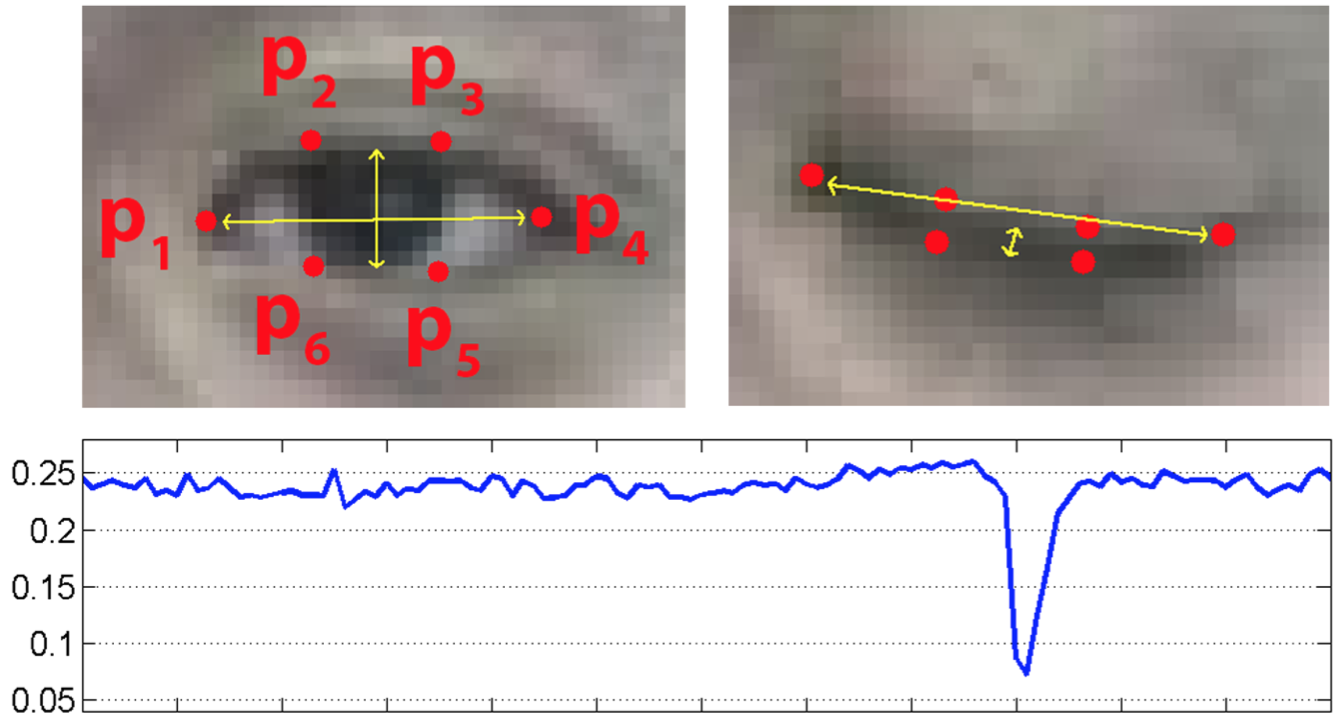
\includegraphics[width=0.49\textwidth]{ear.png}
    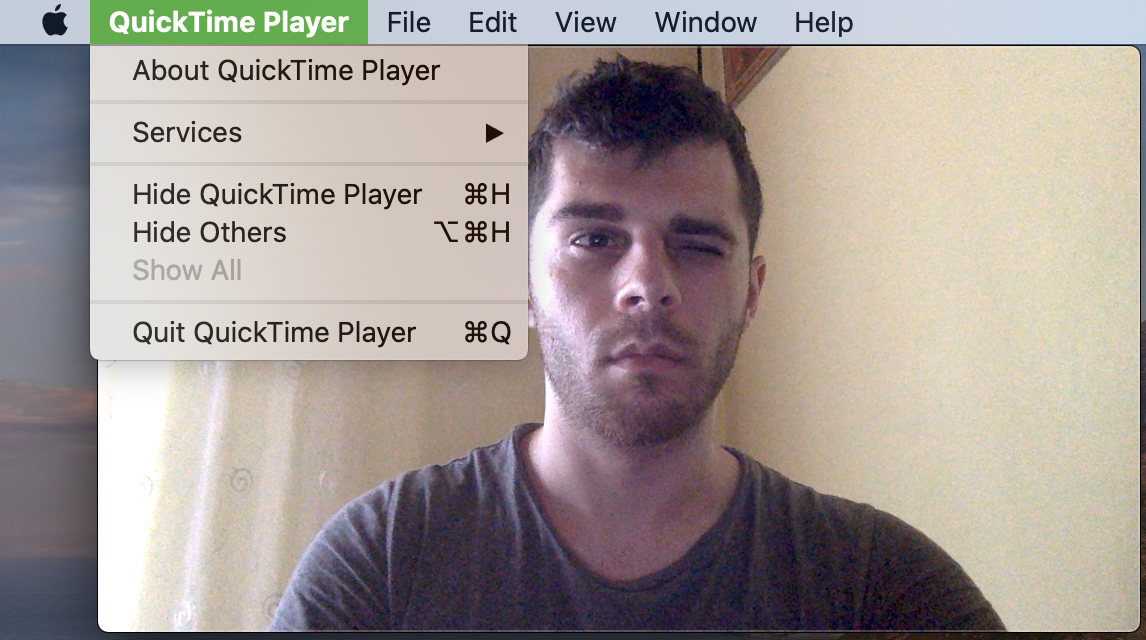
\includegraphics[width=0.49\textwidth]{left_click.png}
    \caption{Simularea apăsării butonului stâng de pe mouse folosind valoarea EAR. Prima imagine ilustrează detectarea clipirii și este preluată din \cite{blink_detection}}
\end{figure}